\subsection{Scenario 1}

\noindent The problem to be optimized can be expressed as

\begin{equation}\label{eq:opt.prob1}
\begin{split}
    U(x) &= u(c_0) + \beta \cdot \sum_{i=1}^{N} \pi_i \cdot u(c_{1,i}) \quad \rightarrow \quad \max_{x}\\
    \text{\textit{subject to}} &\\
    c_0 & = K - x \cdot p_0, \\
    c_{1,i} & = x \cdot d_{1,i}, \\
    x & \geq 0.
\end{split}   
\end{equation}

\bigskip

\noindent The Lagrangian associated to this optimization problem is

\begin{equation}\label{eqn:lagr_risky}
\begin{split}
    L(\lambda_i, x, \mu) = u(c_0) + \beta \cdot \sum_{i=1}^{N} & \pi_i \cdot u(c_{1,i}) + \lambda_0 \cdot (K-x \cdot p_0-c_0) + \\ & + \sum_{i=1}^{N} \lambda_i \cdot (x \cdot d_{1,i} - c_{1,i}) + \mu \cdot x.
\end{split}
\end{equation}

\bigskip

\noindent The first order conditions of optimality are formulated as follows:

\begin{minipage}{0.45\textwidth}
    \begin{subequations}\label{eq:lagr1,lambda_0}
    \begin{align}
        \frac{\partial L}{\partial \lambda_0} = K - xp_0 - c_0 & \geq 0 \\
        \lambda_0 & \geq 0 \\
        \lambda_0 \cdot \frac{\partial L}{\partial \lambda_0} & = 0
    \end{align}
    \end{subequations}
\end{minipage}\hfill
\begin{minipage}{0.45\textwidth}
    \begin{subequations}\label{eq:lagr1,lambda_i}
    \begin{align}
        \frac{\partial L}{\partial \lambda_i} = x d_{1,i} - c_{1,i} & \geq 0\\
        \lambda_i & \geq 0\\
        \lambda_i \cdot \frac{\partial L}{\partial \lambda_i} & = 0
    \end{align}
    \end{subequations}    
\end{minipage}\hfill

\bigskip

\begin{minipage}{0.45\textwidth}
    \begin{subequations}\label{eq:lagr1,c_0}
    \begin{align}
        \frac{\partial L}{\partial c_0} = u'(c_0) - \lambda_0 & \leq 0\\
        c_0 & \geq 0 \\
        c_0 \cdot \frac{\partial L}{\partial c_0} & = 0
    \end{align}
    \end{subequations}
\end{minipage}\hfill
\begin{minipage}{0.45\textwidth}
    \begin{subequations}\label{eq:lagr1,c_{1,i}}
    \begin{align}
        \frac{\partial L}{\partial c_{1,i}} = \beta \pi_i u'(c_{1,i}) - \lambda_i & \leq 0\\
        c_{1,i} & \geq 0 \\
        c_{1,i} \cdot \frac{\partial L}{\partial c_{1,i}} & = 0
    \end{align}
    \end{subequations}    
\end{minipage}\hfill

\bigskip

\begin{minipage}{0.45\textwidth}
    \begin{subequations}\label{eq:lagr1,mu}
    \begin{align}
        \frac{\partial L}{\partial \mu} = x & \geq 0\\
        \mu & \geq 0 \\
        \mu \cdot \frac{\partial L}{\partial \mu} & = 0
    \end{align}
    \end{subequations}    
\end{minipage}\hfill
\begin{minipage}{0.45\textwidth}
    \begin{subequations}\label{eq:lagr1,x}
    \begin{align}
        \frac{\partial L}{\partial x} = -\lambda_0 p_0 + \sum_{i=1}^{N} \lambda_i d_{1,i} & \leq 0\\
        x & \geq 0 \\
        x \cdot \frac{\partial L}{\partial x} & = 0
    \end{align}
    \end{subequations}    
\end{minipage}\hfill

\bigskip
\bigskip

\noindent In section \ref{INADA} it has already been stated that the INADA condition is satisfied. Hence, consumption must be larger than zero today $c_0$ and tomorrow $c_{1,i}$. Therefore, the investor will always choose to consume some share of his capital immediately and invest some in order to have consumption tomorrow. \\

\noindent From $c_0$ being strictly positive and the optimality condition \eqref{eq:lagr1,c_0} one can see that 

\begin{equation}\label{eq:opt.cond.lambda_0}
    \lambda_0 = u'(c_0),
\end{equation}

\bigskip

\noindent which is always larger than zero according to equation \eqref{eq:ut.func.derivatives}. Therefore, the first constraint of the optimization problem \eqref{eq:opt.prob1} must be binding (see condition \eqref{eq:lagr1,lambda_0}), which has already been assumed. \\
The Lagrange-multiplier $\lambda_0$ indicates the marginal utility with respect to the available capital $K$: A small increase in capital $\Delta K$ causes a small gain in utility $\Delta u = \lambda_0 \cdot \Delta K$.\\

\noindent Similarly, it can be shown through the optimality condition \eqref{eq:lagr1,c_{1,i}} that

\begin{equation}\label{eq:opt.cond.lambda_i}
    \lambda_i = \beta \pi_i u'(c_{1,i}).
\end{equation}

\bigskip

\noindent The Lagrange-multiplier $\lambda_i$ corresponds to the rate of change of the total utility with respect to $c_{1,i}$ and is again strictly positive, as long as the probability $\pi_i$ is larger than zero. Otherwise this state can be neglected anyway. \\
From condition \eqref{eq:lagr1,lambda_i} follows that also the second boundary condition of the optimization problem \eqref{eq:opt.prob1} is binding. Therefore, also the number of units of the risky investment $x$ purchased by the investor is strictly positive. The Lagrange-multiplier $\mu$ must be zero according to condition \eqref{eq:lagr1,mu}.\\
Furthermore, condition \eqref{eq:lagr1,x} with $x > 0$ leads to

\begin{equation}
    -\lambda_0 p_0 + \sum_{i=1}^{N} \lambda_i d_{1,i} = 0.
\end{equation}

\bigskip

\noindent Applying the equations \eqref{eq:opt.cond.lambda_0} and \eqref{eq:opt.cond.lambda_i} one ultimately gets

\begin{equation}\label{eq:result1}
\begin{split}
    u'(c_0) p_0 & = \beta \sum_{i=1}^{N} \pi_i u'(c_{1,i}) d_{1,i},\\
    c_0 & = K - x p_0,\\
    c_{1,i} & = x d_{1,i}, \quad \forall i.
\end{split}
\end{equation}

\bigskip

\noindent Thus, the optimal investment and consumption strategy is determined by the marginal utility of consumption. Today's consumption is a function of tomorrow's payoffs, state probabilities, the price and the discount factor \citep{dangl2021notes}. \\

\noindent Considering the derivative of the utility function $u'(c) = c^{-\gamma}$, it is possible to transform equation \eqref{eq:result1} as follows:

\begin{equation}\label{eq:spendings-ratio1}
\begin{split}
    &c_0^{-\gamma}p_0 = \beta \sum_{i=1}^{N} \pi_i (c_{1,i})^{-\gamma} d_{1,i}\\
    &\Rightarrow \quad c_0^{-\gamma} = \beta \sum_{i=1}^{N} \pi_i (xd_{1,i})^{-\gamma} \frac{d_{1,i}}{p_0}\\
    &\Rightarrow \quad \bigg( \frac{c_0}{xp_0} \bigg)^{-\gamma} = \beta p_0^{\gamma-1} \sum_{i=1}^{N} \pi_i d_{1,i}^{1-\gamma}\\
    &\Rightarrow \quad \frac{xp_0}{c_0} = \beta^{\frac{1}{\gamma}} p_0^{1- \frac{1}{\gamma}} \bigg( \sum_{i=1}^{N} \pi_i d_{1,i}^{1-\gamma} \bigg) ^{\frac{1}{\gamma}}
\end{split}
\end{equation}

\bigskip

\noindent Hence, the ratio of capital spent on the investment and consumed immediately $\frac{xp_0}{c_0}$ is independent of the amount of initial capital, $K$, and does only depend on the discount factor, the price, the state probabilities and tomorrow's payoffs of the investment.\\

\noindent A smaller discount factor $\beta$ causes the investor to invest less into tomorrow, due to the smaller weight placed on the utility gathered at $t=1$.\\

\noindent The relation between the price $p_0$ and the spending ratio $\frac{xp_0}{c_0}$ depends on the constant relative risk aversion $\gamma$.\\
For $\gamma = 1$ the spending-proportion is independent of the price. A less risk averse agent ($0 < \gamma < 1$) responds to a higher price by spending less on the investment. An investor with higher relative risk aversion ($\gamma > 1$) responds to a higher price by investing more and consuming less.\\
The infinitely risk averse agent would always purchase the same number of investment units $x$, i.e., the spending-ratio is directly proportional to the price $p_0$.\\

\noindent In order to model the influence of a dividend change, the dividends in each state are multiplied by a factor $k$:

\begin{equation*}
    d_{1,i} = k \cdot \tilde{d}_{1,i}
\end{equation*}

\bigskip

\noindent This results in a multiplication of the expected gross return $E(d_{1,i}/p_0)$ by $k$, as well as the standard deviation. Thus, the higher $k$, the higher the expected gross return. An increase in $k$ affects the investment decision in two ways:

\begin{enumerate}[label=(\alph*)]
    \item With higher return from investment, there is an incentive to consume less today in order to profit more from the higher return.
    \item With higher return from investment, there is also an incentive to consume more today, because a lower investment is sufficient to have enough consumption tomorrow \citep{dangl2021notes}.
\end{enumerate}

\noindent After substitution in equation \eqref{eq:spendings-ratio1} the factor $k$ can be separated and it can be seen that the spending ratio $\frac{xp_0}{c_0}$ is proportional to $k^{\frac{1}{\gamma}-1}$.

\begin{equation}
\begin{split}
    \frac{xp_0}{c_0} = \beta^{\frac{1}{\gamma}} \cdot p_0^{1- \frac{1}{\gamma}} \cdot & \bigg( \sum_{i=1}^{N} \pi_i \tilde{d}_{1,i}^{1-\gamma} \bigg) ^{\frac{1}{\gamma}} \cdot k^{\frac{1}{\gamma}-1}\\
    & \\
    \Rightarrow & \quad \frac{xp_0}{c_0} \sim k^{\frac{1}{\gamma}-1}
\end{split}
\end{equation}

\bigskip

\noindent When risk aversion is low ($0<\gamma<1$), an increase in dividends has the same effect as a price cut, because both are an increase in gross return: the investor will spend more on the investment and consume less immediately. Effect (a) is dominant.\\

\noindent Equally, when risk aversion is high ($\gamma>1$), an increase in gross return causes the spending ratio to decrease and more is consumed immediately. Now effect (b) is dominating.\\

\noindent At $\gamma = 1$, the investor is called "myopic" \citep{dangl2021notes}. In this case the investment decision is independent of the expected returns, as well as the price $p_0$.

\bigskip

\begin{figure}[h!]
    \centering
    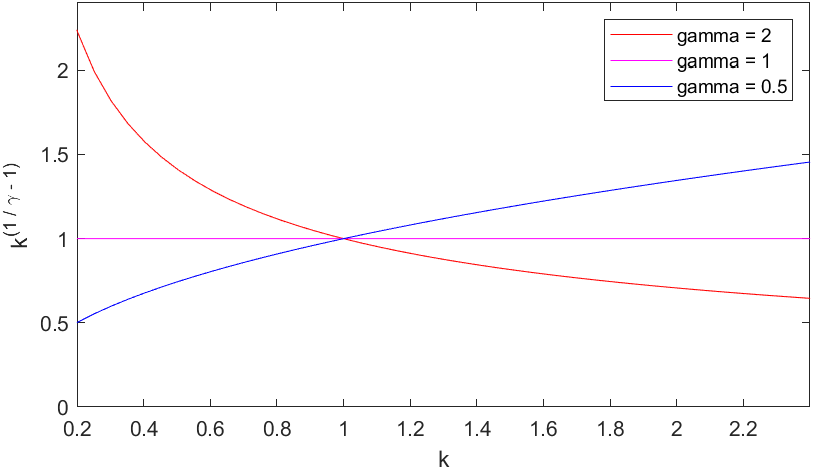
\includegraphics[width=0.7\textwidth]{files/matlab - spending_ratio-k-graph.png}\label{fig:k-spend_ratio}
    \caption{Effect of factor k on the spendings ratio}
\end{figure}

\bigskip

\noindent However, investment behavior is not only determined by the magnitude of the dividends, but also by their variance. I want to illustrate this effect, which is referred to as "mean preserving spread" \citep{rothschild1970mps}, with a simplified model with only two states at $t=1$, $d_{1,1} \leq d_{1,2}$.\\
The probability of occurrence of the two states shall be equal $\pi_1 = \pi_2 = 0.5$. The dividends in each state are chosen such that the expected return $\sum_{i=1}^{2} \pi_i d_{1,i}$ remains constant at $1$. The abscissa is to describe the spread $s$ of the dividends, modelled as $1-\frac{d_{1,1}}{d_{1,2}}$:

\begin{equation*}
\begin{split}
    d_{1,1} &= \frac{2-2s}{2-s}\\
    d_{1,2} &= \frac{2}{2-s}
\end{split}
\end{equation*}

\bigskip

\noindent At $s=0$ the dividends $d_{1,1}$ and $d_{1,2}$ are equal, there is no spread. As $s$ approaches $1$, $d_{1,1}$ converges towards $0$, while the expected return must remain constant. Therefore, $d_{1,2}$ approaches $2$. At $s=1$ the spread is at its maximum. Meanwhile, $\beta$ and $p_0$ are both fixed at a value of $1$.\\


\begin{figure}[h!]
    \centering
    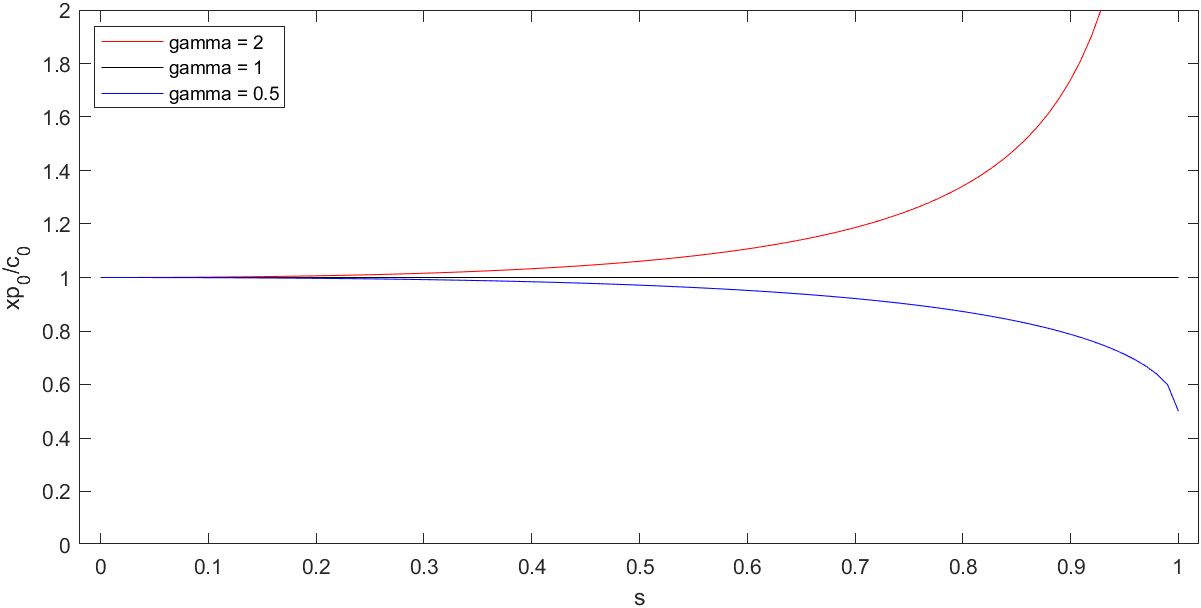
\includegraphics[width=0.7\textwidth]{files/matlab - mean preserving spread s.png}\label{fig:s-dividends-spread}
    \caption{Effect of mean preserving spread on the spending ratio}
\end{figure}

\bigskip

\noindent This diagram shows that the influence of \lq\lq mean preserving spread" depends on the relative risk aversion $\gamma$:\\
At $\gamma = 1$, the spending ratio once again remains unaffected by the dividends.\\
An investor with a strong risk aversion $(\gamma>1)$ reacts to an increase in dividend spread with a larger investment portion. This is due to the fact, that the highly risk averse investor fears to be left with little or even no consumption at $t=1$. A larger investment should offset this risk.\\
Conversely, when risk aversion is lower than one, a large dividend spread results in more immediate consumption. The slightly risk averse investor does not consider it necessary to hedge against the risk of low returns because the minimum utility is limited (see page \pageref{isoel.ut.f:limits}). More of the capital is spent on immediate consumption because its resulting utility is certain.


\vspace{10mm}

\noindent An alternative approach to determine the optimum is by substitution of $c_0$ with $K-xp_0$ in the original optimization problem \eqref{eq:opt.prob1}:

\begin{equation}
    f(x) = u(K - xp_0) + \beta \sum_{i=1}^{N} \pi_i u(c_{1,i}).
\end{equation}

\bigskip

\noindent The model, which originally was a model in $c_0$ and uncertain $c_1$, can now be described with a one-dimensional function in $x$. The optimum can be found through differentiation and solving for the maximum:

\begin{equation}
    \frac{d}{dx} f(x) = -p_0 u'(K - xp_0) + \beta \sum_{i=1}^{N} \pi_i u'(c_{1,i}) d_{1,i} = 0
\end{equation}

\bigskip

\noindent This leads to the same result as obtained in equation \eqref{eq:result1}. Since the objective function is globally concave in $x$ and $y$ and all constraints are linear in these investment decisions, 2nd-order optimality conditions are satisfied, i.e., the determined candidate $(x^*,y^*)$ maximizes the investors utility \citep[p. 131]{dangl2022bwopt}.\\

\noindent It is noticeable that by taking the derivative with respect to $xp_0$ instead of $x$, one side of the equation yields exactly the derivative of the total utility function $U(c_0, c_1)$ from equation \eqref{eq:opt.prob1} with respect to $c_0$:

\begin{equation}
    \frac{\partial U}{\partial c_0} = u'(c_0) = MU_{c_0}
\end{equation}

\bigskip

\noindent The other side of the equation equals the derivative of the total utility with respect to $xp_0$:

\begin{equation}
    \frac{\partial U}{\partial (xp_0)} = \beta \sum_{i=1}^{N} \pi_i u'(c_{1,i}) \frac{d_{1,i}}{p_0} = MU_{xp_0}
\end{equation}

\bigskip

\noindent Thus, the marginal utilities with respect to $c_0$ and $xp_0$ must be equal, i.e., the increase in utility caused by an additional unit of capital must be the same, whether it is consumed immediately or invested.\\
Otherwise it would be possible to gain utility by simply transferring a small amount of capital from the investment option with lower marginal utility to the asset with higher marginal utility:

\begin{align*}
    \text{if} & \quad MU_{c_0} >(<) MU_{xp0}:\\
    \\
    \Delta U & \cong -MU_{xp0} \cdot \Delta K + MU_{c_0} \cdot \Delta K\\
    & = \Delta K \cdot (MU_{c_0} - MU_{xp0}) >(<) 0. 
\end{align*}

\bigskip

\noindent This would be contrary to the fundamental properties of an optimum. Therefore, in the maximum point the marginal utilities with respect to $c_0$ and $xp_0$ must be equal.

\vspace{10mm}

\noindent Other interesting aspects of this problem can be determined by rearranging equation \eqref{eq:result1} as follows:

\begin{equation}\label{eq:pricing_eq1}
    p_0 = \sum_{i=1}^{N} \pi_i \beta \frac{u'(c_{1,i})}{u'(c_0)} d_{1,i}
\end{equation}

\bigskip

\noindent This equation is the "central asset pricing formula" 
\citep[p. 6]{cochrane2001asset}. The right side is called the expected discounted value of the asset's payoff. If the price does not match this function of payoffs, there exists a change in the investor’s investment strategy such that the the associated change in consumption would improve the investor’s total expected utility. The term

\begin{equation}\label{eq:stochastic_disc_fac}
    m_i = \beta \frac{u'(c_{1,i})}{u'(c_0)}
\end{equation}

\bigskip

\noindent is called the stochastic discount factor. It can be thought of as a weight placed on the different possible states, similar to the discount factor $\beta$, but state dependent, regarding differences in (marginal) utility.\\
For example, if there was a risk neutral investor ($\gamma = 0$), then the stochastic discount factor would be equal to $\beta$:

\begin{equation*}
    u'(c) = 1 \quad \Rightarrow \quad m_i = \beta.
\end{equation*}

\bigskip

\noindent Therefore, the investor's equilibrium price exactly matches the discounted expected dividend

\begin{equation*}
    p_0(\gamma = 0) =  \beta \sum_{i=1}^{N} \pi_i d_{1,i}.
\end{equation*}

\bigskip

\noindent A risk averse agent has different stochastic discount factors $m_i$ for different states. For a high level of consumption, tomorrow's marginal utility is low (due to saturation). Thus, a lower weight is placed on the states with higher dividends. States with a relatively low level of consumption have a disproportionately high weight \citep{dangl2021notes}.\\

\noindent In other words, to a risk averse investor, the probability of a state $i$ appears higher than it actually is if the dividend $d_{1,i}$ is lower compared to the others. Conversely, states with higher dividend receive lower weight.






